\chapter{AFABL Programmer Study}\label{ch:afabl-study}

%% Basili and colleagues have conducted many experiments and written extensively about the role of experiments in software engineering research and the kinds of knowledge that can be gained from experimentation \cite{basili2007role,basili1986a-experimentation}. In Table \ref{tab:basili-framework} we fit our experiments within Basili's framework.

%% Definition
%% ---
%% Motivation - assess advantage of AFABL, validate language-integrated RL
%% Object - a programming language applied to a particular kind of programming task
%% Purpose -evaluate
%% Perspective - user (of the programming language)
%% Domain - programmer
%% Scope - single project by single programmer

%% Planning
%% ---
%% Design - Randomized
%% Criteria - size, complexity
%% Measurement - Metric validation, subjective reflection

%% Operation
%% ---
%% Preparation - pilot study
%% Execution - data collection: online-delivered programming tasks
%% Analysis - quantitative: comparison of complexity metrics, complexities; qualitative

%% Interpretation
%% ---
%% Statistical framework - t-test
%% Extrapolation -
%% Impact


AFABL supports a declarative style in which the agent programmer specifies which states are desirable and undesirable, but not how the agent should choose actions to pursue or avoid those states. Action selection logic is derived automatically by reinforcement learning algorithms that the AFABL programmer never sees. AFABL also provides agent-based software abstractions that permit code to be reused in new domains. This reuse is one of the things we mean by adaptivity: existing AFABL code can adapt to new domains without modifying the code. In this chapter we report the results of a programmer study to quantify the value of AFABL's agent programming abstractions.

\section{Experiments}

Programmers were randomly assigned to two equally-sized groups based on their demographics (see Appendix \ref{ch:programmer-study} for details): one group used Scala without AFABL first -- the Scala-first group -- and the other group used AFABL first -- the AFABL-first group.  Each group completed two programming tasks using Scala and AFABL in the order determined by their group.  For each task the programmers were asked to write elegant code that meets the requirements of the task as quickly as possible, balancing the quality of their solutions with time.  The idea was to get a good solution quickly, not a perfect solution in a long time.

\subsection{Task 1: Bunny-Food-Wolf}\label{sec:task1}

\begin{figure}[h]

\begin{center}
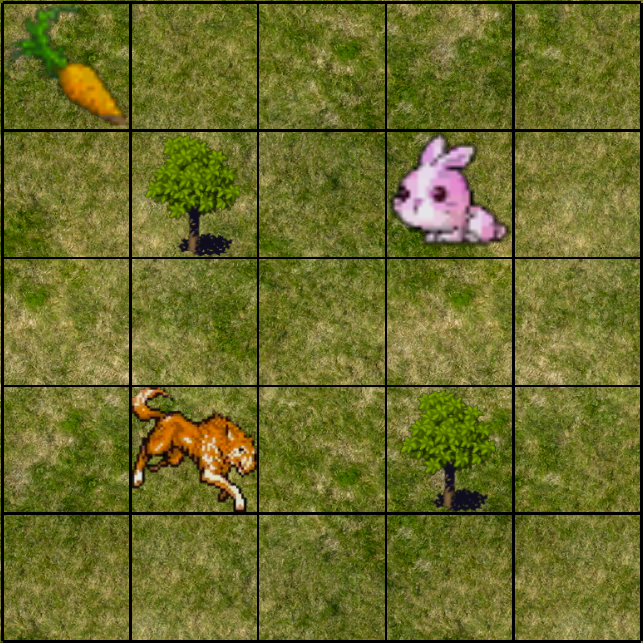
\includegraphics[height=2.4in]{bunny.png}
\end{center}


\caption{In the grid world above, the bunny must pursue two goals simultaneously: find food and avoid the wolf.  The bunny may move up, down, left, or right.  When it finds food it consumes the food and new food appears elsewhere in the grid world, when it meets the wolf it is eaten and ``respawns'' elsewhere.}
\label{fig:bunny-picture}
\end{figure}

In this task each programmer wrote an agents that control a bunny character in a simple world, depicted in Figure~\ref{fig:bunny-picture}.  The bunny world works as follows:

\begin{itemize}

\item The bunny world is a discrete grid of cells.  The bunny, wolf, and food each occupy one cell.

\item During each time step the bunny may move north, south, east, or west -- this is the bunny agent's action set.

\item Every two time steps the wolf moves towards the bunny.

\item If the bunny moves to the cell currently occupied by the food, the agent should be written to recognize this fact and give the agent an appropriate reward signal. In any case the simulation assumes food is ``eaten'' and new food appears elsewhere.

\item If the wolf moves to the cell currently occupied by the bunny it eats the bunny and the bunny ``respawns'' in a new location.

\end{itemize}

Programmers were asked to write bunny agents that meet the wolf as little as possible and eat as much food as possible. \added[id=v3]{The bunny's percepts are complete state descriptions: the locations of the bunny and the wolf.}

\subsection{Task 2: Mating Bunny}\label{sec:task2}

In this task each programmer wrote a bunny agent for a world that is identical to the world in Task 1 except that the bunny must also find mates.  This world includes one static  potential mate that behaves similarly to the food.  When the bunny finds the potential mate, the simulation assumes that the bunny has ``mated,'' the mate disappears, and another potential mate appears elsewhere.  The simulation runs as in Task 1, and the scorer additionally keeps track of how many mates the bunny finds.  As in Task 1, programmers were asked to write bunny agents that meet the wolf as little as possible, eat as much food as possible, and find as many mates as possible. \added[id=v3]{As in Task 1, the bunny's percepts are complete state descriptions: the locations of the bunny, the wolf and the mate.}

\subsection{Provided Code}

Study participants were given starter code so they could focus on writing the behavior of their agents. We provided the world for each task and the files in which to write their code. Participants were also given general documentation for AFABL but assumed to already be proficient in Scala.

Figure \ref{fig:scala-task1-provided} shows the code given to participants for the Scala bunny on Task 1. Figure \ref{fig:afabl-task1-provided} shows the code given to participants for the AFABL bunny on Task 1. The {\tt BunnyWorld}, {\tt BunnyState}, and {\tt BunnyAction} classes were also provided. It was up to participants to write state abstraction classes if they chose to do so.


\begin{figure}[!h]
\begin{center}

\begin{lstlisting}[language=Scala]
class ScalaBunny1 extends Agent[BunnyState, BunnyAction.Value]
    with Task1Scorer {

  // Your code goes in the body of this method. This method defines
  // your agent's behavior, that is, what action it takes in a given
  // state. The last expression in this method must be a
  // BunnyAction.  You may create as many helper functions as you
  // like, but please do not alter any of the provided code.
  def getAction(state: BunnyState, shouldExplore: Boolean = false) = {

    // This is a stub to make the code compile. Please
    // replace this with your code.
    BunnyAction.Up
  }
}
\end{lstlisting}

\caption{Starter Scala code provided to participants for Task 1.}
\end{center}
\label{fig:scala-task1-provided}
\end{figure}


\begin{figure}[!h]
\begin{center}

\begin{lstlisting}[language=Scala]
object AfablTask1 {

  // Use this val in your agent definitions.
  val bunnyWorld = new BunnyWorld

  // Please place all of your AFABL code for Task 1 in this singleton
  // object.


  // Your solution must assign your AFABL bunny agent for Task 1 to
  // the val afablBuny1.
  val afablBunny1 = ???
}
\end{lstlisting}

\caption{Starter AFABL code provided to participants for Task 1.}
\end{center}
\label{fig:afabl-task1-provided}
\end{figure}


The provided code for Task 2 was identical to the provided code for Task 1, except for the names of the files. For Task 2 participants were encouraged to copy code from Task 1 if they found it helpful, or to use any objects defined for Task 1 that would be helpful, such as behavior modules. As we discuss below, reusing code was straightforward for the AFABL agents but not for the Scala agents. As in Task 1, it was up to participants to write state abstraction classes if they chose to do so, but they could reuse any state abstraction classes written for Task 1.

Each task had a main method which ran the agents in the world to evaluate their performance.

\section{Quantitative Analysis}

We analyzed the submissions of study participants to compare Scala agents to AFABL agents in terms of code size, time spent writing Scala versus AFABL agents, the complexity of Scala versus AFABL agent code, and the performance of the agents on the assigned tasks.

\subsection{Code Size}

The size of a code base is often correlated with the level of effort required to write or understand the code. We computed the number of lines of code for each agent, not including comments.

\subsection{Time}

Study participants used the IntelliJ IDEA IDE with a plug-in that we wrote especially for this study. The plug-in recorded timestamps each time the editor tab with Task 1 or Task 2 files gained or lost the focus. We processed these logs to add up the time deltas between gaining and losing focus as an indication of the time programmers spent writing the code for each bunny agent.

\subsection{Cyclomatic Complexity}

We computed a complexity measure for all the submitted bunny agents. For Scala code we employed the simplified McCabe cyclomatic complexity measure \cite{mccabe1976complexity}:

\begin{equation}
v = \pi + 1
\end{equation}

where $v$ is the complexity score and $\pi$ is the number of predicates in decision structures.

\subsection{Performance}

Each programmer's Scala bunny and AFABL bunny were run for 1000 time steps and their average scores recorded. The score is based on how much food the bunny eats and how many times the bunny is eaten by the wolf for Task 1, and additionally how many times the bunny mates for Task 2. The score is normalized by the number of steps to indicate a sort of ``happiness index,'' a ratio of rewards to lifespan. This score happens to correspond to the measure used to validate Arbi-Q in Chapter \ref{ch:arbiq} to facilitate comparison between programmer authored agents and the performance of the algorithms we implemented for our reformulated MRL. It is important to note, however, that our aim here is not to achieve optimal performance but to create a programming system that makes it easy to write agents that achieve good performance.

\subsection{Typical Task 1 Submissions}

\begin{figure}[!h]
\begin{center}

\begin{lstlisting}[language=Scala]
class ScalaBunny1 extends Agent[BunnyState, BunnyAction.Value]
    with Task1Scorer {

  def getAction(state: BunnyState, shouldExplore: Boolean = false) = {
    if (wolfNearFood(state))
      moveAwayFromWolf(state)
    else
      moveTowardFood(state)
   }

  def wolfNearFood(state: BunnyState) = {
    val wolfToFood = sqrt(pow(state.food.x - state.wolf.x, 2) +
                          pow(state.food.y - state.wolf.y, 2))
    val bunnyToFood = sqrt(pow(state.food.x - state.bunny.x, 2) +
                           pow(state.food.y - state.bunny.y, 2))
    wolfToFood < bunnyToFood
  }

  def moveTowardFood(state: BunnyState) = {
    if (state.food.x > state.bunny.x)
      BunnyAction.Right
    else if (state.food.x < state.bunny.x)
      BunnyAction.Left
    else if (state.food.y < state.bunny.y)
      BunnyAction.Up
    else
      BunnyAction.Down
  }

  def moveAwayFromWolf(state: BunnyState) = {
    if (state.wolf.x < state.bunny.x)
      BunnyAction.Right
    else if (state.wolf.x > state.bunny.x)
      BunnyAction.Left
    else if (state.wolf.y > state.bunny.y)
      BunnyAction.Up
    else
      BunnyAction.Down
  }
}
\end{lstlisting}

\caption{Typical Scala submission for Task 1.}
\end{center}
\label{fig:scala-task1-submission}
\end{figure}

Figure \ref{fig:scala-task1-submission} shows a typical Scala submission for Task 1. The action selection strategy is about as simple as possible. For example, there is no determination of where the wolf is in relation to the bunny and food other than distance. If the wolf is closer to the food than the bunny, move away from the wolf, otherwise move toward to the food. The agent does not distinguish between cases where the wolf is between the wolf and the food, or if the wolf is closer but sufficiently far away. One could imagine writing code to calculate the projection of the wolf's position onto the line between the bunny and the food to determine a safe closure rate for the wolf. However, this simple strategy is all that is needed to achieve nearly optimal results. This Scala-only bunny agent achieves an average performance score of 0.54, the same as the AFABL bunny.

\begin{figure}[!h]
\begin{center}

\begin{lstlisting}[language=Scala]
  case class FindFoodState(bunny: Location, food: Location)
  val findFood = AfablModule(
    world = bunnyWorld,
    stateAbstraction = (worldState: BunnyState) => {
      FindFoodState(worldState.bunny, worldState.food)
    },
    moduleReward = (moduleState: FindFoodState) => {
      if (moduleState.bunny == moduleState.food) 1.0
      else -0.1
    }
  )

  case class AvoidWolfState(bunny: Location, wolf: Location)
  val avoidWolf = AfablModule(
    world = bunnyWorld,
    stateAbstraction = (worldState: BunnyState) => {
      AvoidWolfState(worldState.bunny, worldState.wolf)
    },
    moduleReward = (moduleState: AvoidWolfState) => {
      if (moduleState.bunny == moduleState.wolf) -0.1
      else 0.1
    }
  )

  val afablBunny1 = AfablAgent(

    world = bunnyWorld,

    modules = Seq(findFood, avoidWolf),

    agentLevelReward = (state: BunnyState) => {
      if (state.bunny == state.wolf) 0.0
      else if (state.bunny == state.food) 1.0
      else 0.5
    }
  )
\end{lstlisting}

\caption{Typical AFABL submission for Task 1.}
\end{center}
\label{fig:afabl-task1-submission}
\end{figure}

Figure \ref{fig:afabl-task1-submission} shows a typical AFABL submission for Task 1. As in our earlier examples, the AFABL bunny is composed of behavior modules for finding food and avoiding the wolf. The AFABL documentation contained tips for reward authoring in modules and at the agent level.

The AFABL solution to Task 1 contains 31 lines of code and has a cyclomatic complexity of 5 (4 predicates in decision structures). The Scala solution to Task 1 uses 34 lines of code and has a cyclomatic complexity of 8 (7 predicates in decision structures). Both programs achieve the same nearly optimal level of performance with scores of ~0.54. \added[id=v3]{Optimal performance was determined by running GM-Sarsa/Q-decomposition on the problem, which has been shown by Russell and Zimdars to be optimal \cite{russell2003q-decomposition}.}

\subsection{Typical Task 2 Submissions}

\begin{figure}[!h]
\begin{center}

\begin{lstlisting}[language=Scala]
class ScalaBunny2 extends Agent[BunnyState, BunnyAction.Value]
    with Task2Scorer {

  def getAction(state: BunnyState, shouldExplore: Boolean = false) = {

    if ((distance(state.wolf, state.food) < distance(state.food, state.bunny))
      || distance(state.wolf, state.mate) < distance(state.mate, state.bunny))
      moveAwayFromWolf(state)
    else if (distance(state.bunny, state.food) < distance(state.bunny, state.mate))
      moveToward(state.bunny, state.food)
    else
      moveToward(state.bunny, state.mate)
  }

  def distance(a: Location, b: Location) = {
    sqrt(pow(a.x - b.x, 2) + pow(a.y - b.y, 2))
  }

  def moveToward(from: Location, to: Location) = {
    if (to.x > from.x)
      BunnyAction.Right
    else if (to.x < from.x)
      BunnyAction.Left
    else if (to.y > from.y)
      BunnyAction.Up
    else
      BunnyAction.Down
  }

  def moveAwayFromWolf(state: BunnyState) = {
    if (state.wolf.x < state.bunny.x)
      BunnyAction.Right
    else if (state.wolf.x > state.bunny.x)
      BunnyAction.Left
    else if (state.wolf.y > state.bunny.y)
      BunnyAction.Up
    else
      BunnyAction.Down
  }
}
\end{lstlisting}

\caption{Typical Scala submission for Task 2.}
\end{center}
\label{fig:scala-task2-submission}
\end{figure}

Figure \ref{fig:scala-task2-submission} shows a typical Scala solution for Task 2. While the Scala solution to Task 2 is more complex than the Scala solution to Task 1, it uses only one more line of code -- 35 -- due to refactoring of common logic. Of course, this refactoring took extra time and without the refactoring the line count and likely the cyclomatic complexity would have been higher.

\begin{figure}[!h]
\begin{center}

\begin{lstlisting}[language=Scala]
  case class FindMateState(bunny: Location, mate: Location)
  val findMate = AfablModule(
    world = bunnyWorld,
    stateAbstraction = (state: BunnyState) => {
      FindMateState(state.bunny, state.mate)
    },
    moduleReward = (state: FindMateState) => {
      if (state.bunny == state.mate) 1.0
      else -0.1
    }
  )

  // Your solution must assign your AFABL bunny agent for Task 2 to
  // the val afablBuny2.
  val afablBunny2 = AfablAgent(

    world = bunnyWorld,

    modules = Seq(AfablTask1.findFood, AfablTask1.avoidWolf, findMate),

    agentLevelReward = (state: BunnyState) => {
      if (state.bunny == state.wolf) 0.0
      else if (state.bunny == state.food) 1.0
      else if (state.bunny == state.mate) 1.0
      else 0.5
    }
  )
\end{lstlisting}

\caption{Typical AFABL submission for Task 2.}
\end{center}
\label{fig:afabl-task2-submission}
\end{figure}

Figure \ref{fig:afabl-task2-submission} shows typical AFABL code for Task 2. Notice that the {\tt findFood} and {\tt avoidWolf} modules from Task 1 have been reused directly. This works because the world, {\tt BunnyWorld}, is the same. In Task 1 the bunny was ignoring the mate. In Task 2 we adapt the bunny to find the mate, and all we need to do is add a {\tt findMate} module and add a line to the {\tt agentLevelReward} function so that the agent will also value finding mates.

The AFABL solution to Task 2 contains 21 lines of code due to reuse of modules from Task 1, and has the same cyclomatic complexity of 5 (4 predicates in decision structures) even though the agent is solving a more complex problem. Even with the refactoring of common logic in Task 2 the Scala solution has a higher cyclomatic complexity of 10 (9 predicates in decision structures), which McCabe says is the maximum allowable cyclomatic complexity for a testable, maintainable software module \cite{mccabe1976complexity}. Finally, the performance of the Scala solution to Task 2 decreases to 0.48, while the AFABL solution continues to achieve the same nearly optimal 0.54. With additional work perhaps the Scala agent's performance on Task 2 could have been improved, but the point here is that AFABL agents are easier to write, easier to adapt to new domains, have less complex code, and perform well without requiring a great deal of effort beyond choosing reward signals.

\subsection{Quantitative Results}

\begin{center}
\begin{table}[h]
\caption{Quantitative results of Scala agent code versus AFABL agent code on Task 1. p-value is for comparison of means between samples of unequal variances (Welch's t-test \cite{welch1947generalization}). A p-value of less than .05 mean that the difference in means is statistically significant at the 95\% significance level, i.e. we reject $H_0: \mu_1 = \mu_2$ and conclude that the means are different. Power is the probability that we reject the null hypothesis $H_0$ when it is in fact false, given the sample size, variance, and significance level of 95\% ($\alpha = .05$).}
\label{tbl:task1-results}

\begin{center}
\begin{tabular}{|l|r|r|r|r|}\hline
Task 1 & Scala Mean & AFABL Mean & p-value & Power \\\hline
Time in seconds & 1511.45 & 1780.91 & 0.47 & 0.11\\
Lines of code & 39.33 & 31.20 & 0.22 & 0.85\\
Complexity & 10.80 & 5.27 & 0.01 & 1.00\\
Performance & 0.44 & 0.53 & 0.02 & 0.73\\
\hline
\end{tabular}

\end{center}
\end{table}
\end{center}

\begin{center}
\begin{table}[h]
\caption{Quantitative results of Scala agent code versus AFABL agent code on Task 2. p-value is for comparison of means between samples of unequal variances (Welch's t-test \cite{welch1947generalization}). A p-value of less than .05 mean that the difference in means is statistically significant at the 95\% significance level, i.e. we reject $H_0: \mu_1 = \mu_2$ and conclude that the means are different. Power is the probability that we reject the null hypothesis $H_0$ when it is in fact false, given the sample size, variance, and significance level of 95\% ($\alpha = .05$).}

\begin{center}
\begin{tabular}{|l|r|r|r|r|}\hline
Task 2 & Scala Mean & AFABL Mean & p-value & Power \\\hline
Time in seconds & 797.82 & 626.73 & 0.53 & 0.10\\
Lines of code & 41.67 & 39.20 & 0.62 & 0.08\\
Complexity & 11.27 & 8.20 & 0.05 & 0.95\\
Performance & 0.48 & 0.54 & 0.03 & 0.98\\
\hline
\end{tabular}

\end{center}
\label{tbl:task2-results}
\end{table}
\end{center}


Overall results for Task 1 are summarized in Table \ref{tbl:task1-results}. Overall results for Task 2 are summarized in Table \ref{tbl:task2-results}. All but one of the study programmers created good AFABL agents. One programmer failed to understand the right way to write the reward function and therefore got very poor performance with their AFABL agents. The data do not show statistically significant differences in time or lines of code, but for the same amount of time and number of lines of code AFABL solutions were less complex and performed better. We also believe that the AFABL results for time are unreliable because programmers left their editors open while they were reading documentation on AFABL. So the time measures for AFABL solutions include programming time and the time spent learning AFABL. Given this fact, the similarity in time between Scala and AFABL solutions indicates that AFABL programs are indeed quicker to write, but we cannot say that with statistical certainty.

\subsubsection{Programmer Demographics}

We collected demographic data from each programmer, including professional programming experience (work experience), the largest program personally written (code experience), agent programming proficiency, Scala proficiency, level of education, and major. Almost all participants were undergraduate students, and all participants were computer science majors except for one electrical engineering major who was an experienced professional programmer proficient in Scala. The only categories in which there was a nearly 50\% split were code experience and agent programming experience, so we compared these splits to get a sense of how programming proficiency affected their results.

Interestingly, the only metric on which experienced and novice coders had statistically significant difference was in lines of code for the Scala solution to Task 1. This result makes some sense given that Scala is an expressive language with terse idioms available to experienced programmers. The lack of differences in other metrics suggest that the agent programming problem was simply to small to reveal differences in programmer proficiency.

\begin{center}
\begin{table}[h]
\caption{Comparison of novice vs. experienced coder results. p-value is for comparison of means between samples of unequal variances (Welch's t-test \cite{welch1947generalization}). A p-value of less than .05 mean that the difference in means is statistically significant at the 95\% significance level, i.e. we reject $H_0: \mu_1 = \mu_2$ and conclude that the means are different. Power is the probability that we reject the null hypothesis $H_0$ when it is in fact false, given the sample size, variance, and significance level of 95\% ($\alpha = .05$).}

\begin{center}

\begin{tabular}{|l|r|r|r|r|}\hline
Afabl Task 1 & Coding Novice Mean & Experienced Coder Mean & p-value & Power\\\hline
Time in Seconds & 2071.00 & 1539.17 & 0.39 & 0.12\\
Lines of Code & 31.43 & 31.00 & 0.69 & 0.07\\
Complexity & 5.00 & 5.50 & 0.35 & 0.24\\
Performance & 0.55 & 0.51 & 0.30 & 0.26\\
\hline
\end{tabular}


\begin{tabular}{|l|r|r|r|r|}\hline
Afabl Task 2 & Coding Novice Mean & Experienced Coder Mean & p-value & Power\\\hline
Time in Seconds & 470.20 & 757.17 & 0.30 & 0.18\\
Lines of Code & 40.43 & 38.12 & 0.62 & 0.08\\
Complexity & 8.29 & 8.12 & 0.75 & 0.06\\
Performance & 0.55 & 0.54 & 0.45 & 0.11\\
\hline
\end{tabular}


\begin{tabular}{|l|r|r|r|r|}\hline
Scala Task 1 & Coding Novice Mean & Experienced Coder Mean & p-value & Power\\\hline
Time in Seconds & 1487.60 & 1531.33 & 0.92 & 0.05\\
Lines of Code & 25.71 & 51.25 & 0.04 & 0.67\\
Complexity & 8.14 & 13.12 & 0.13 & 0.33\\
Performance & 0.44 & 0.44 & 0.99 & 0.05\\
\hline
\end{tabular}


\begin{tabular}{|l|r|r|r|r|}\hline
Scala Task 2 & Coding Novice Mean & Experienced Coder Mean & p-value & Power\\\hline
Time in Seconds & 470.20 & 757.17 & 0.30 & 0.18\\
Lines of Code & 40.43 & 38.12 & 0.62 & 0.08\\
Complexity & 8.29 & 8.12 & 0.75 & 0.06\\
Performance & 0.55 & 0.54 & 0.45 & 0.11\\
\hline
\end{tabular}

\end{center}
\label{tbl:code-experience}
\end{table}
\end{center}


As the results in Table \ref{tbl:agent-experience} show, agent programming experience had no effect on any of the programming metrics. This results suggests that simple agent problems are readily soved with AFABL, and that the agent problems in the study were not sufficiently complex to bring out differences in agent programming experience.

\begin{center}
\begin{table}[h]
\caption{Comparison of results from programmers no agent programming experience vs programmers with some agent programming experience. p-value is for comparison of means between samples of unequal variances (Welch's t-test \cite{welch1947generalization}). A p-value of less than .05 mean that the difference in means is statistically significant at the 95\% significance level, i.e. we reject $H_0: \mu_1 = \mu_2$ and conclude that the means are different. Power is the probability that we reject the null hypothesis $H_0$ when it is in fact false, given the sample size, variance, and significance level of 95\% ($\alpha = .05$).}

\begin{center}

\begin{tabular}{|l|r|r|r|r|}\hline
Afabl Task 1 & Agent Novice Mean & Some Agent Exp Mean & p-value & Power\\\hline
Time in Seconds & 1770.00 & 1787.14 & 0.98 & 0.05\\
Lines of Code & 31.83 & 30.78 & 0.45 & 0.14\\
Complexity & 5.67 & 5.00 & 0.36 & 0.29\\
Performance & 0.55 & 0.51 & 0.34 & 0.19\\
\hline
\end{tabular}


\begin{tabular}{|l|r|r|r|r|}\hline
Afabl Task 2 & Agent Novice Mean & Some Agent Exp Mean & p-value & Power\\\hline
Time in Seconds & 552.50 & 669.14 & 0.71 & 0.06\\
Lines of Code & 40.67 & 38.22 & 0.57 & 0.08\\
Complexity & 8.17 & 8.22 & 0.92 & 0.05\\
Performance & 0.55 & 0.54 & 0.54 & 0.09\\
\hline
\end{tabular}


\begin{tabular}{|l|r|r|r|r|}\hline
Scala Task 1 & Agent Novice Mean & Some Agent Exp Mean & p-value & Power\\\hline
Time in Seconds & 1717.50 & 1393.71 & 0.56 & 0.09\\
Lines of Code & 40.83 & 38.33 & 0.84 & 0.05\\
Complexity & 11.17 & 10.56 & 0.87 & 0.05\\
Performance & 0.43 & 0.44 & 0.81 & 0.06\\
\hline
\end{tabular}


\begin{tabular}{|l|r|r|r|r|}\hline
Scala Task 2 & Agent Novice Mean & Some Agent Exp Mean & p-value & Power\\\hline
Time in Seconds & 552.50 & 669.14 & 0.71 & 0.06\\
Lines of Code & 40.67 & 38.22 & 0.57 & 0.08\\
Complexity & 8.17 & 8.22 & 0.92 & 0.05\\
Performance & 0.55 & 0.54 & 0.54 & 0.09\\
\hline
\end{tabular}

\end{center}
\label{tbl:agent-experience}
\end{table}
\end{center}


\subsection{Qualitative Results}

\begin{figure}[h!]
\begin{tabular}{cc}\\
  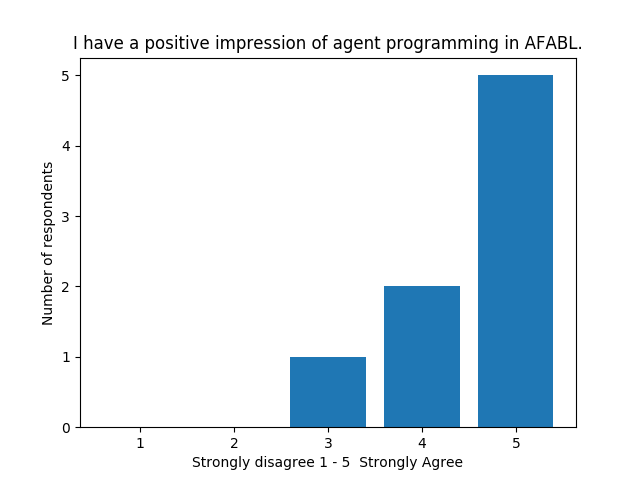
\includegraphics[height=2.5in]{afabl-impression.png} & 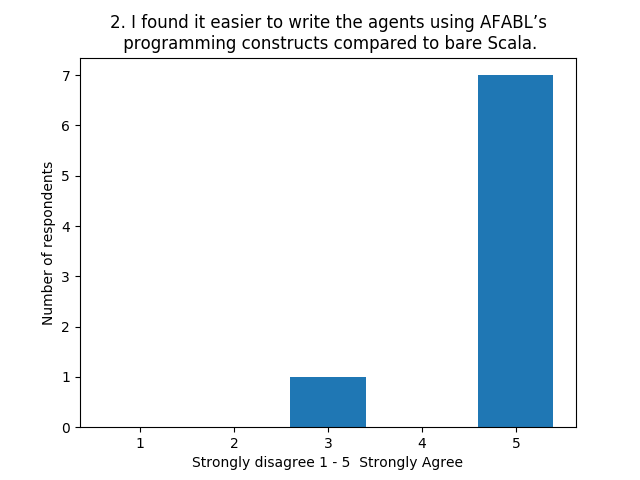
\includegraphics[height=2.5in]{afabl-easier-overall.png} \\
  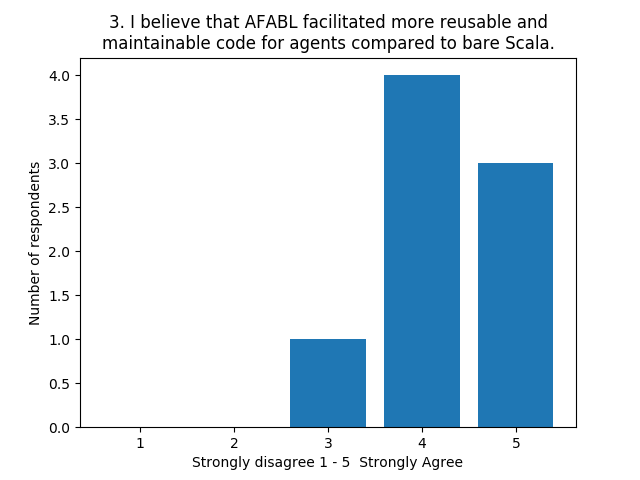
\includegraphics[height=2.5in]{afabl-better-maintenance.png} & 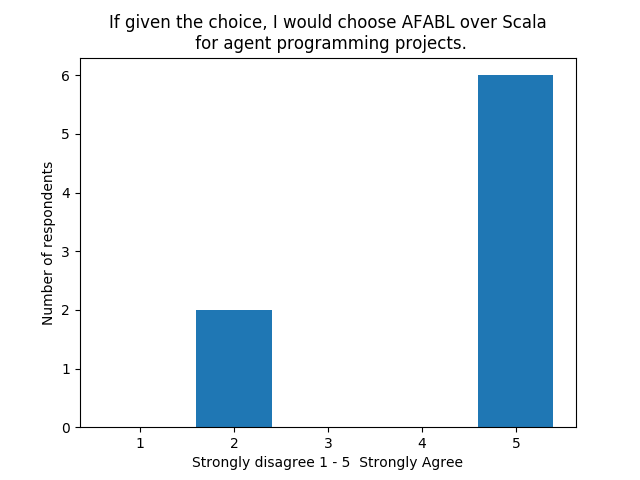
\includegraphics[height=2.5in]{afabl-choice.png} \\
  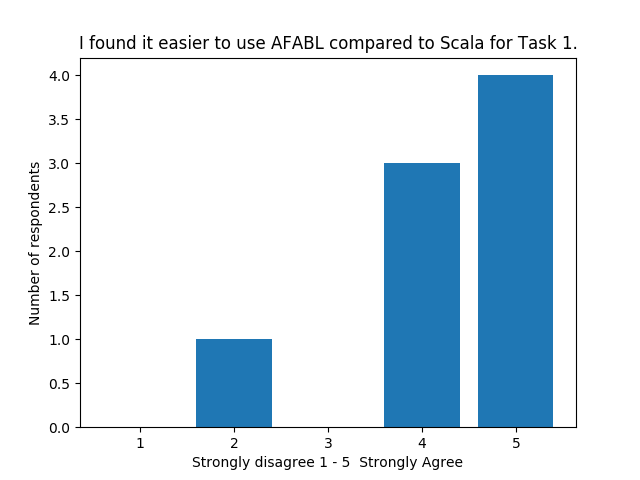
\includegraphics[height=2.5in]{afabl-easier-task1.png} & 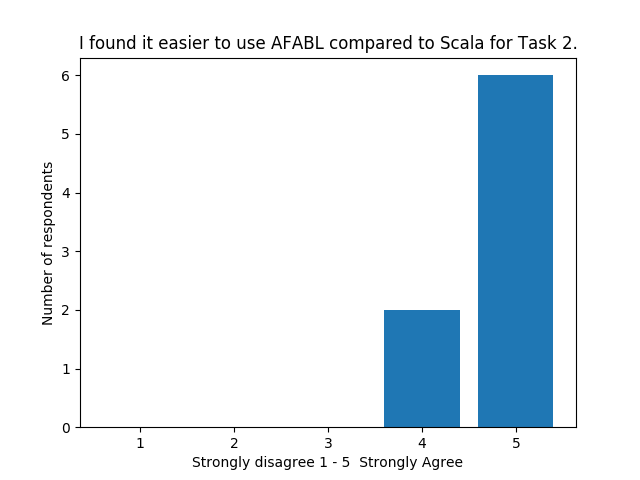
\includegraphics[height=2.5in]{afabl-easier-task2.png} \\\hline
\end{tabular}
\caption{Responses to Likert-scale question on reflection survey.}
\label{fig:likert-responses}
\end{figure}

Programmers responded to a questionnaire to give their impressions of agent programming in AFABL versus agent programming in Scala. Here we summarize the responses of the eight participants who were not TAs of the principal investigator. Figure \ref{fig:likert-responses} shows that programmers had a positive response to AFABL. The most interesting responses of these is for the question ``If given the choice, I would choose AFABL over Scala for agent programming projects.'' Although every programmer found AFABL to be easier than Scala for Task 2, and almost all programmers found AFABL easier for Task 1, some of the study participants were very experienced Scala programmers who would still prefer the familiarity of Scala. The programmer who reported that they would choose Scala over AFABL did report for Task 2 that they found it easier to adapt their AFABL agent to Task 2 after they had developed some basic knowledge of AFABL.

\subsubsection{Internal Validity of Reflection Survey}

The Cronbach alpha coefficient measures the correlation between the answers to questions that measure the same construct and is given by:

\[
\alpha = \frac{k}{k - 1} \times (1 - \frac{s_{T}^{2} - \sum s_{I}^{2}}{s_{T}^{2}})
\]

where
\begin{itemize}
\item $s_T^2$ is the total variance of all the items (questions) for a construct
\item $s_I^2$ is the variance of an individual item, and
\item $k$ is the number of items.
\end{itemize}

We evaluated the internal consistency of the survey by calculating the Cronbach alpha coefficients for the following constructs:

\begin{enumerate}

\item User satisfaction with Scala for agent programming tasks.
\begin{itemize}
\item Questions 1 and 3
\item Cronbach alpha: 1.38
\end{itemize}

\item User satisfaction with AFABL for agent programming tasks.
\begin{itemize}
\item  Questions 2 and 4
\item Cronbach alpha: 1.35
\end{itemize}

\item User preference for AFABL over Scala for agent programming tasks.
\begin{itemize}
\item Questions 5 and 7
\item Cronbach alpha: 1.28
\end{itemize}

\end{enumerate}

Since all Cronbach alpha scores were above 0.7, we may consider the reflection survey to be reliable.

\subsubsection{Free Response Questions}

Two of the questions on the survey allowed for free responses. These responses are listed below, again, only for non-TAs.

{\bf What was it about AFABL that made Task 1 easier or harder?}

\begin{itemize}
\item I didn't have to put so much thought into the mechanics of moving and distance calculation, and didn't have to think about priorities.
\item The choice of going towards to food or avoiding the wolf is tricky. Should you only avoid the wolf when it's adjacent? 2 Squares away? what exactly does it mean to avoid? Answering these questions is hard, but expressing the rewards and punishments for getting food and meeting the wolf is easy. AFABL did not require me to express these domain-specific problems, instead it learned based on the rewards and costs what policy is optimal.
\item No need to explicitly compare locations, calculate distances or balance separate goals.
\item Easier because it only asks for important parts of the specific domain, more difficult as I don't know how different goals interact and I don't know why my end score was lower in AFABL or what changes improve a score.
\item While learning AFABL had some overhead for Task 1, being able to program in terms of rewards and punishments was much more intuitive than coding an algorithm from scratch that may or may not be correct.
\item I've written agents similar to my Scala agent in the past, so it took much less new thought to develop it, whereas the AFABL agent was conceptually and structurally very different from anything I've written before, and were therefore harder to approach.
\item You simply define success and failure scenarios; there's no dealing with weighting different values and that makes it MUCH easier to work with, as a programmer.
\item There was no need to define the movement algorithm
\end{itemize}

{\bf What was it about AFABL that made Task 2 easier or harder?}

\begin{itemize}
\item All I had to do was add a 3rd module which was very much like FindFood.
\item Same arguments as 1, but now there's the mate. I actually found that I could treat the mate exactly as a food source by adding another module very similar to the food module. The problem then became how to maximize the total reward by playing around with the module-level rewards and the agent-level rewards. If it were very important to find good reward values, one could run some optimization program on the rewards. It's worth mentioning that if I were faced with this problem, I would feel more comfortable running an optimization algorithm than writing my own domain-specific agent behavior. AFABL would pair nicely with a solver that optimizes on rewards.
\item The design of independent modules made adding an additional module/goal trivial.
\item Both were pretty easy to add 1 more goal. But in Scala I copied and pasted. In AFABL it was really neat to just import modules from the other file with no effort to integrate them.
\item Being able to just add in another module and tack it onto the agent with AFABL was much easier and more elegant than having to go in and modify existing methods and logic in Scala. Adding the additional functionality with AFABL was much more convenient in this respect.
\item After understanding AFABL to some degree, it was quite easy to modify my existing agent to the new task and thereby receive a good score.
\item You can much more clearly see the similarities between Task 1 and Task 2 in the AFABL version, for one thing. Second, it doesn't require modifying existing code nearly as much as the plain Scala version does. It's a delight to use, and as a programmer at a startup, I would much rather work with this format over what I have to do to work with AWS' Machine Learning program.
\item Too many cases to work on in Scala, hard to figure out whether mating or eating takes importance, takes far less time with AFABL.
\end{itemize}

Many of the answers above mention the reduced time and effort of writing AFABL agents. These answers corroborate our belief that the time tracking in the quantitative section was unreliable due to programmers not following directions to move the focus off their editors while reading documentation, and possible malfunctions in the IntelliJ IDEA plug-in used to automatically track time.

\section{Threats to Validity}

The first threat to validity is sample size -- there were only 16 study participants. Indeed the statistical power calculations for most comparisons indicate that results are inconclusive due to the small sample sizes and large variances in many metrics. However, two core metrics -- complexity and performance -- yielded very high statistical power, supporting our claim that AFABL agent programs are simpler to write than their non-AFABL equivalents, and that it takes less effort to get good performance from AFABL agents.

The second threat is problem size. The tasks that programmers were given were smaller than typical software engineering tasks. Given the difficulty of getting programmers to work for hours writing programs for a study, and the further challenge of finding Scala programmers, the problem size had to be limited. We believe that the insights are still valid because the chief differences between AFABL agent programs and traditional programs are the control-flow complexity and the additional effort required to adapt agent programs to more complex domains. As our results showed, the small tasks were sufficient to show these differences.

The final threat to validity is the fact that 8 of the 16 study participants were teaching assistants for the principal investigator. This fact may have biased them towards writing better AFABL solutions in order to help me show positive results. However, as Table \ref{tbl:tas-vs-non-tas} shows, the data do not show that the TAs' results differed from the non-TAs' results. Again, due to small samples sizes the statistical power of these comparisons is low, but nevertheless we cannot show a statistically significant difference between the results of TAs and non-TAs.

\begin{center}
\begin{table}[h]
\caption{Comparison of TA results versus non-TA results. p-value is for comparison of means between samples of unequal variances (Welch's t-test\cite{welch1947generalization}). A p-value of less than .05 mean that the difference in means is statistically significant at the 95\% significance level, i.e. we reject $H_0: \mu_1 = \mu_2$ and conclude that the means are different. Power is the probability that we reject the null hypothesis $H_0$ when it is in fact false, given the sample size, variance, and significance level of 95\% ($\alpha = .05$).}

\begin{center}
\begin{tabular}{|l|r|r|r|r|}\hline
Afabl Task 1 & TA Mean & Non-TA Mean & p-value & Power\\\hline
Time in Seconds & 1620.00 & 1733.33 & 0.86 & 0.05\\
Lines of Code & 31.38 & 31.12 & 0.82 & 0.06\\
Complexity & 5.00 & 5.50 & 0.35 & 0.26\\
Performance & 0.51 & 0.54 & 0.42 & 0.19\\
\hline
\end{tabular}


\begin{tabular}{|l|r|r|r|r|}\hline
Afabl Task 2 & TA Mean & Non-TA Mean & p-value & Power\\\hline
Time in Seconds & 686.83 & 552.00 & 0.62 & 0.08\\
Lines of Code & 41.75 & 38.25 & 0.47 & 0.11\\
Complexity & 8.38 & 8.12 & 0.61 & 0.08\\
Performance & 0.55 & 0.54 & 0.19 & 0.26\\
\hline
\end{tabular}


\begin{tabular}{|l|r|r|r|r|}\hline
Scala Task 1 & TA Mean & Non-TA Mean & p-value & Power\\\hline
Time in Seconds & 1520.67 & 1462.17 & 0.89 & 0.05\\
Lines of Code & 36.88 & 40.12 & 0.80 & 0.06\\
Complexity & 10.62 & 11.12 & 0.88 & 0.05\\
Performance & 0.46 & 0.42 & 0.47 & 0.11\\
\hline
\end{tabular}


\begin{tabular}{|l|r|r|r|r|}\hline
Scala Task 2 & TA Mean & Non-TA Mean & p-value & Power\\\hline
Time in Seconds & 686.83 & 552.00 & 0.62 & 0.08\\
Lines of Code & 41.75 & 38.25 & 0.47 & 0.11\\
Complexity & 8.38 & 8.12 & 0.61 & 0.08\\
Performance & 0.55 & 0.54 & 0.19 & 0.26\\
\hline
\end{tabular}

\end{center}
\label{tbl:tas-vs-non-tas}
\end{table}
\end{center}


\section{Conclusion}

As you can see from the similarity of the submission in Figure \ref{fig:afabl-task1-submission} to our explanatory example, most AFABL bunny agents look the same. There is one obvious way to implement a bunny agent that must pursue multiple goals. This uniformity is desirable. As Tim Peters says in the Zen of Python \cite{peters2004zen}, ``There should be one-- and preferably only one --obvious way to do it.'' The similarity in most AFABL solutions to a particular modular agent programming problem is an indication that AFABL provides the right abstractions for adaptive agent programming. \added[id=v3]{This regularity results from exploiting the structure of certain kinds of agent programming problems. In the next chapter we discuss the kinds of problems for which AFABL is well-suited and those for which it is less well-suited.}
